\documentclass{article}
\usepackage{arxiv}

\usepackage[utf8]{inputenc}
\usepackage[T1]{fontenc}
\usepackage{hyperref}
\usepackage{url}
\usepackage{booktabs}
\usepackage{array}
\usepackage{amsmath}
\usepackage{amsfonts}
\usepackage{microtype}
\usepackage{siunitx}
\usepackage{graphicx}
\usepackage{longtable}
\usepackage{pgfplots}
\usepgfplotslibrary{statistics}
\pgfplotsset{compat=1.18}
\setlength\LTleft{0pt}
\setlength\LTright{0pt}

\title{YouSpeed Technical Report: System Architecture, Jurisdiction Handling, Bundle Generation, and Lightweight Matching Benchmarks for Offline Smartphone Speed-Limit Assistance}

\author{
  Raphael Volz \\
  Pforzheim University \\
  \texttt{raphael.volz@hs-pforzheim.de}
}

\begin{document}
\maketitle

\begin{abstract}
This technical report documents the current YouSpeed system for offline smartphone speed-limit assistance. The system couples regional OpenStreetMap-derived bundles, on-device area-context lookup, bounded local map matching, and jurisdiction-aware warning logic across two mobile clients: the iPhone release-track application and the Android internal alpha. The report treats four connected questions. First, it documents the current local-first architecture, bundle contract, and mobile-client feature scope. Second, it characterizes regulation handling and maxspeed provenance, including a Germany-specific provenance decomposition and a cross-country explicit-tag analysis over 45 European extracts. Third, it describes the actual bundle-generation and iterative-update pipeline, including country selection, regional sharding, delta-pack publication, and the current v3 database schema. Fourth, it reports the benchmark evidence for four runtime data architectures, an all-log complexity ladder of causal matcher stages, and five named deployable matcher experiments on closed-loop replay corpora. S3, a single-file spatially indexed database, remains the stable data-layer choice. The all-log complexity ladder is used to measure what each added matcher mechanism contributes on the current log inventory; it is not itself the deployment ranking. The deployable runtime comparison now separates two frontiers. The corridor-aware final remains the strongest replay-quality profile on the present corpora. Experiment M2, a nearest plus street-ref continuity heuristic, is the strongest lightweight profile and attains the highest current internal score \(S\) because it keeps the smaller 108.5 MiB bundle, near-baseline latency, and very low oscillation. Experiment M3 reintroduces connected-candidate filtering to suppress disconnected bridge and tunnel competitors, but it does not improve on M2 on the present corpora, so the current lightweight evidence still favors the branch that can omit \texttt{way\_links}. Both consumer apps still execute the corridor-aware \texttt{corridorHMM} runtime, while the smaller connected baseline remains an internal benchmark reference, M2 becomes a concrete lightweight alternative, M3 isolates the value of reintroducing graph connectivity into that lightweight family, and the raw mini-HMM profile remains a benchmark-only live candidate inside the richer corridor family. Within that deployed matcher family, the all-log hindsight screen still shows that added complexity is not monotone: the raw mini-HMM stage provides the strongest aggregate causal operating point on fixed candidate windows, but the closed-loop replay benchmark rejects it as a direct consumer-app replacement. The current system is therefore asymmetric in other respects: the bundle and data architecture are stable, jurisdiction-aware warning logic is broader than jurisdiction-aware legal-default inference, and matcher selection is driven by closed-loop deployable evidence rather than by offline hindsight scores alone.
\end{abstract}

\keywords{intelligent speed assistance \and offline-first \and OpenStreetMap \and map matching \and mobile GIS \and smartphone systems}

\section{Introduction}
Intelligent speed assistance (ISA) is now a regulatory requirement for new vehicle types in the European Union, yet the installed vehicle base remains far larger than annual new registrations \cite{eu2019_2144,eu2021_1958,eu_mandatory_safety_2024,eurostat_passenger_cars_2026,acea_registrations_2024}. This keeps the retrofit question open: practical speed-limit assistance still needs to run on devices that drivers already carry. Smartphone deployment is therefore relevant not as a theoretical alternative to integrated vehicle systems, but as a current path to broad availability.

YouSpeed addresses that path with a local runtime that keeps map data, area-context lookup, matching, and local correction handling on device. The current codebase spans a shared preprocessing and bundle-publication pipeline, an iPhone client on the launch path, and an Android internal alpha that follows the same bundle contract and the same deployed \texttt{corridorHMM} matcher logic. The engineering question is no longer whether offline inference is possible in principle. The current question is which architecture and which lightweight matching approach best fit the present product and evidence state, while remaining honest about jurisdiction-specific regulation handling and update logistics.

This report reflects that current scope. It does not present a future architecture roadmap, and it does not treat unimplemented crowd synchronization as a central result. Instead, it documents the current system and uses logs as a model-discovery tool toward deployable profiles:
\begin{enumerate}
\item the implemented local-first system architecture and mobile-client feature scope,
\item the way the runtime currently handles jurisdiction identity, warning rules, and speed-limit provenance,
\item the bundle-generation and iterative-update machinery that turns country-scale OSM data into mobile artifacts,
\item four runtime data architectures (S1--S4) for local geospatial lookup,
\item an all-log complexity ladder of causal matching stages that can be embedded into deployable profiles,
\item five named deployable matcher experiments on closed-loop replay corpora, which form the actual deployment comparison.
\end{enumerate}

\section{Related Work}
Map matching has long been framed as a trade-off between geometric simplicity and sequence-aware robustness. The classic survey by \citet{quddus2007} organizes the field into geometric, topological, and probabilistic families. Sequence models then become the dominant answer to noisy and sparse trajectories: the HMM formulation of \citet{newson2009}, ST-matching by \citet{lou2009}, online HMM variants for streaming data \citep{goh2012,he2013}, low-latency path inference by \citet{hunter2014}, and faster precomputed transition schemes such as FMM \citep{yang2018fmm}. These methods demonstrate that later context is powerful, but they also assume a route-inference budget that is larger than the one targeted by the current YouSpeed runtime.

Smartphone-specific work confirms that this literature transfers to consumer sensing, but again usually in a richer probabilistic setting than the one used here. \citet{bierlaire2013smartphone} evaluate a probabilistic matcher directly on smartphone GPS traces, and production engines such as OSRM, Valhalla Meili, and Mapbox expose candidate radiuses, transition controls, and confidence-style outputs as first-class API concepts \citep{osrm_match_service,valhalla_meili,mapbox_map_matching_api}. The present report borrows the scientific lesson that sequence context matters, while keeping the implementation target smaller and fully local.

Recent learning-based work pushes map matching further toward transfer learning, personalization, and adaptation under limited labels. Transformer transfer learning \citep{jin2022transformer}, deep inverse reinforcement learning with multi-intention modeling \citep{safarzadeh2024midirl}, preference-aware HMMs \citep{zhang2025pphmm}, and meta-learning approaches \citep{meng2026mpm} all show that richer models can exploit driver- or context-specific structure. These lines are important context for YouSpeed, but they sit one layer above the current report. The present system still prioritizes bounded local state, auditable heuristics, and direct replay evaluation on device-shaped corpora.

The report also sits close to deployment-oriented packaging work rather than only to inference models. Single-archive spatial delivery formats such as MBTiles and PMTiles show that packaging choices are themselves a mature systems topic \citep{mbtiles_spec,pmtiles_docs}. That point matters because YouSpeed currently compares not only matching logic but also how map data is physically packaged, updated, and routed at country scale. The distinctive contribution of this report is therefore the joint treatment of lightweight matching, jurisdiction handling, mobile-client runtime scope, runtime data architecture, and bundle publication under present product constraints.

\section{System Architecture}
\subsection{Current end-to-end architecture}
The implemented YouSpeed path is local-first and offline-first. OSM snapshot ingestion and preprocessing run off device. The build pipeline emits regional v3 bundles that package road geometries, speed tags, area-context polygons, coverage metadata, and optional corridor tables in a single runtime artifact. Mobile clients load bundled target manifests, choose country or regional artifacts, verify checksums, and activate bundles atomically. During driving, each fix is routed to the best downloaded bundle through a coverage bounding-box prefilter followed by coverage-polygon containment. The selected bundle then executes local lookup, speed derivation, and way selection without a route-level cloud dependency.

Figure~\ref{fig:architecture_scope} summarizes the current paper-scope architecture. The broader cloud corroboration stack that appears in internal architecture documents remains a north-star extension, not the present critical path. The evaluated critical path is snapshot-to-bundle publication, local bundle activation, on-device inference, and editor-mediated export of reviewed local observations.

The benchmark harness sits beside this runtime rather than replacing it. The S1--S4 latency benchmark reuses the same Germany-derived artifacts and query primitives but isolates spatial lookup and area-context retrieval at one fixed probe point. The replay benchmarks reuse the same runtime matcher implementations and logs, but they remove the user-interface lifecycle so that candidate arbitration, tunnel handling, and oscillation behavior can be measured directly.

\begin{figure}[!htbp]
\centering
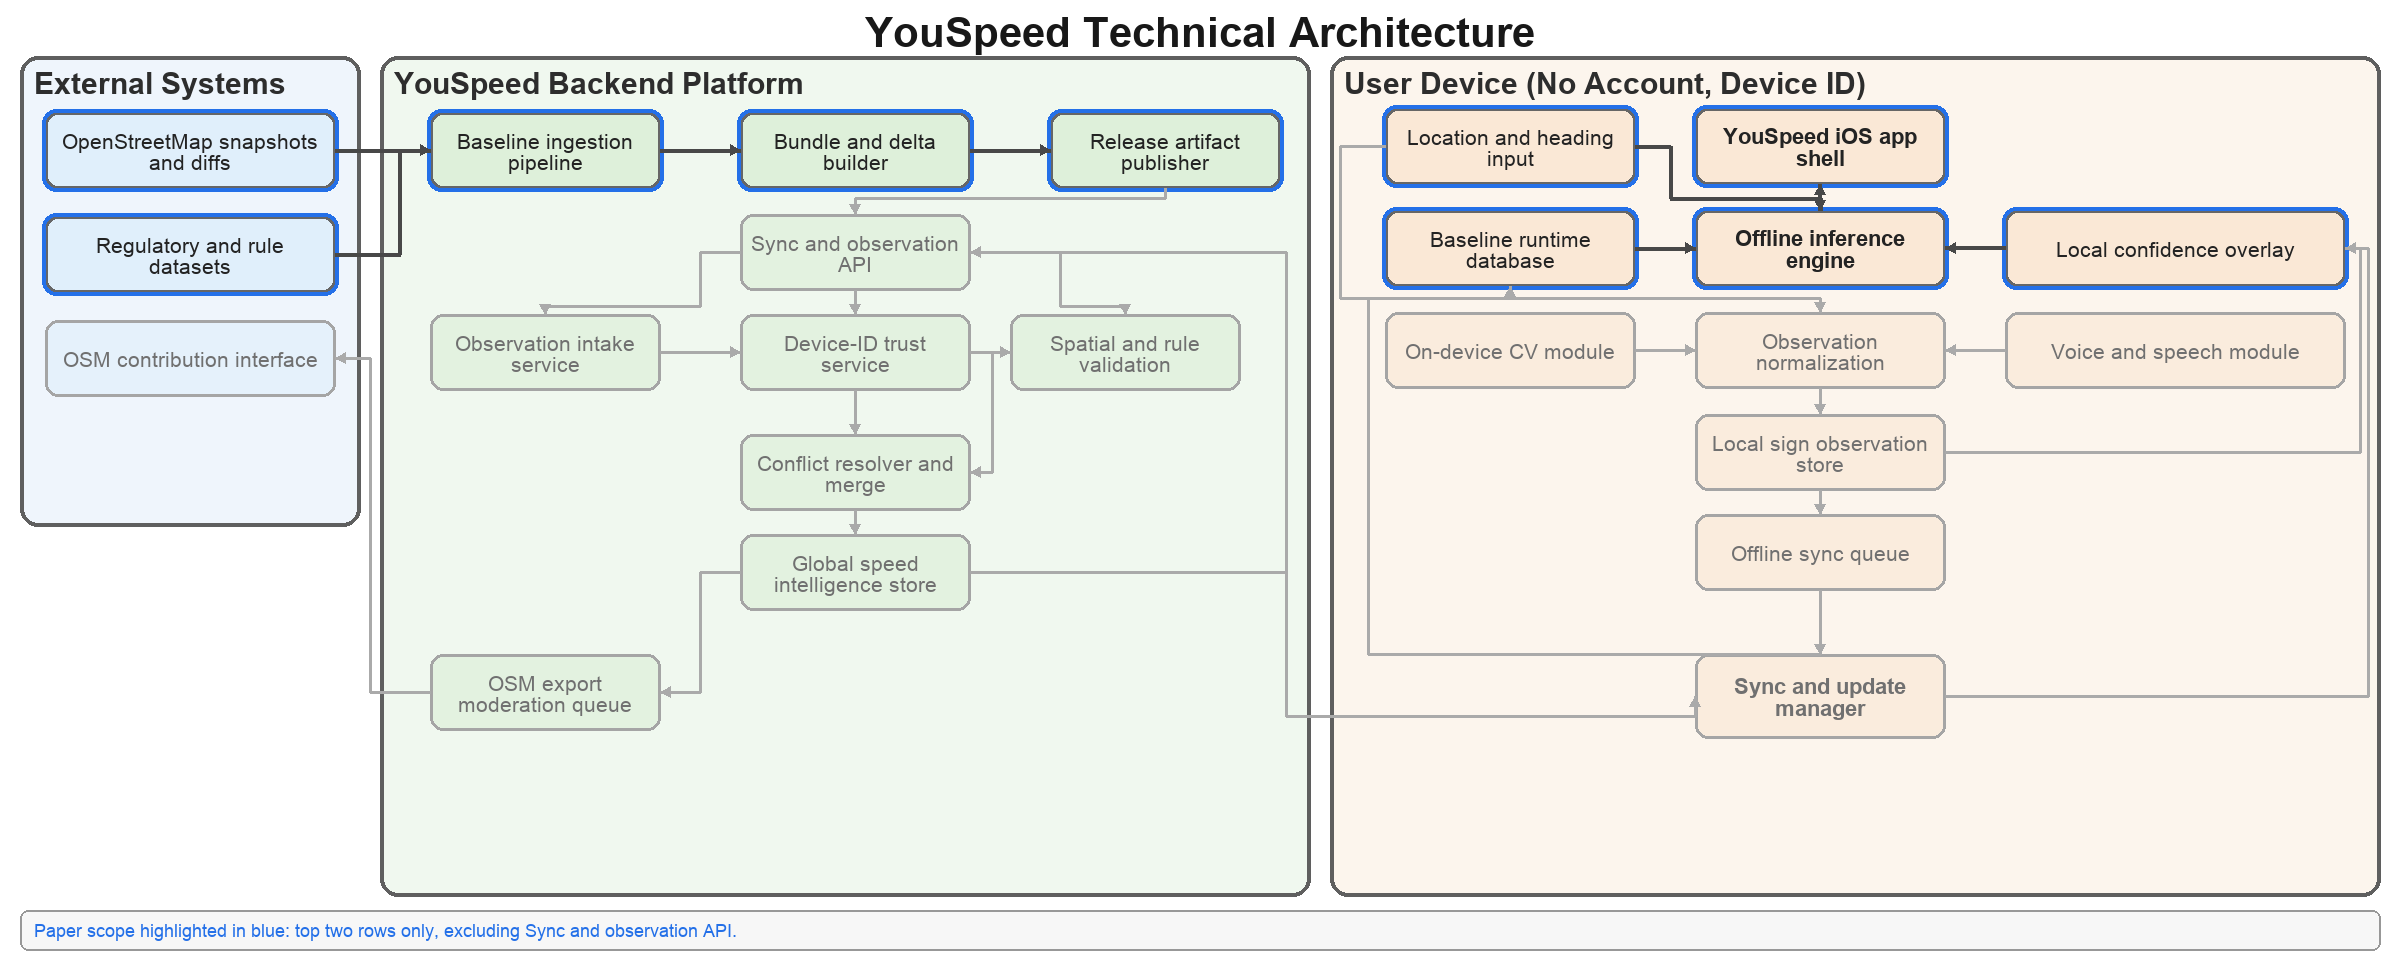
\includegraphics[width=\linewidth]{../share/TECHNICAL_ARCHITECTURE_PAPER_SCOPE.png}
\caption{Current paper-scope system architecture. The implemented critical path is local-first: regional bundle publication, on-device inference, and editor-mediated observation export.}
\label{fig:architecture_scope}
\end{figure}

\subsection{iPhone application}
The iPhone application is the current release-track client. It bootstraps from a bundled Karlsruhe seed, discovers Germany shard manifests from the bundled \texttt{BundleTargets.top10.json} contract, downloads full bundles or verified SQL delta chains when available, assembles multipart database payloads when needed, and activates bundles atomically. The runtime uses plain \texttt{SQLite3} rather than runtime \texttt{mod\_spatialite} loading, with an RTree bounding-box prefilter, polyline distance refinement, optional heading-aware scoring, deterministic tunnel handling, and bundle-coverage routing across downloaded regions.

The same client also carries the current driver-facing feature surface. It presents current speed, inferred limit, street and city context, tunnel state, and penalty-aware overspeed warnings. It captures local speed-limit observations through an on-device speech-recognition workflow, stores them in a review queue, and exports approved proposals as editor-oriented \texttt{.osc} packages rather than publishing directly from the app. The iPhone codebase is also the main source of inspector logs and replay corpora used in the matching benchmarks reported later in this report.

\subsection{Android application}
The Android application is an internal alpha that follows the same bundle and manifest contract as the iPhone client, but it is not the current public release gate. It bootstraps from a bundled seed, derives the same Germany shard endpoints, verifies and activates full bundles or multipart bundle payloads, and mirrors the same local lookup contract. The Android matcher now executes the same deployed \texttt{corridorHMM} path as the iPhone runtime: geometry-first candidate ranking, corridor prefiltering, connected-transition pruning over \texttt{way\_links}, continuity arbitration, short-history mini-HMM re-ranking, a three-way expert gate, and final tunnel or corridor locks backed by \texttt{corridor\_progress} and \texttt{corridor\_pairs}. It also includes a fallback path for Android builds that expose stored RTree tables without exposing the SQLite RTree module at runtime.

The Android alpha emphasizes parity experiments that are useful for architecture validation. It adds spoken overspeed and driving-ban warnings, a bundled German offline Vosk recognizer for local speed capture, SQLite-backed review and export of local observations, debug log export, OSM browser handoff, and emulator or device instrumentation for replay and live bundle bootstrap. This makes Android scientifically relevant even before public launch because it exercises the shared bundle contract and runtime logic under a second mobile platform.

\subsection{Current consumer-app matcher}
The current consumer applications do not run the full seven-stage complexity ladder reported later in the offline benchmark. Both consumer apps now execute the same deployed matcher path: the corridor-aware \texttt{corridorHMM} configuration. The smaller \texttt{connectedBaseline} branch remains available inside the iPhone service as a benchmark and regression reference, and it also remains one of the runtime profiles evaluated later in this report, but it is not the default consumer runtime on either platform.

The deployed matcher is local and bounded rather than route-global. Each fix is resolved from a local candidate window, but the decision carries short history through a \texttt{WayMatchContext} that includes preferred way identity, recent way and street-reference history, recent matched fixes, tunnel approach counters, recent mini-HMM hypotheses, tunnel mode, motorway mode, and active or approaching corridor state. The runtime also consumes three topology side tables from the active bundle. \texttt{way\_links} stores shared-node reachability and shared-reference relations. \texttt{corridor\_progress} stores corridor identity together with entry depth, remaining span, and node counts for tunnel and motorway segments. \texttt{corridor\_pairs} links paired corridor components so that entry and exit chains can be scored consistently across repeated fixes.

\begin{table}[!htbp]
\centering
\scriptsize
\caption{Ordered stages of the deployed \texttt{corridorHMM} matcher in both consumer apps.}
\label{tab:consumer_matcher_stages}
\begin{tabular}{p{2.6cm}p{4.9cm}p{4.5cm}}
\toprule
Stage & Role in the runtime & Main evidence or state source \\
\midrule
Candidate query & Query nearby ways, refine by polyline distance, optionally add heading mismatch, and keep trace features for later gates. & Local candidate set \(C_t\), distance \(d_{t,i}\), heading mismatch \(\Delta \theta_{t,i}\), endpoint proximity. \\
Corridor feasibility gate & Reject candidates incompatible with active or approaching tunnel or motorway corridors, and suppress ambiguous surface-to-tunnel snaps unless recent GPS loss justifies fallback. & \texttt{corridor\_progress}, \texttt{corridor\_pairs}, GPS-loss flag, horizontal-accuracy buffer. \\
Connected road-graph gate & After warmup, remove disconnected transitions and keep only candidates reachable from the recent match state when graph evidence exists. & \texttt{way\_links}, preferred way, matched-fix count. \\
Continuity heuristics & Form preferred-way, same-ref, linked-way, and recent-way classes; then apply bounce suppression, transition promotion, low-speed turn overrides, and conservative continuity holds. & Recent way or ref history, endpoint proximity, speed, heading, graph links. \\
Mini-HMM beam & Score a short beam of candidates together with tunnel or motorway sequence states, using emission penalties plus decayed transition costs from recent hypotheses. The raw mini-HMM stage in Table~\ref{tab:model_benchmark} is the winner of this step before later gates. & Recent hypotheses, corridor state machine, signal evidence, pair-aware transition penalties. \\
Three-way expert gate & When the sequence state is still surface-like, arbitrate between current, lowest-distance, and lowest-endpoint experts; veto same-ref bounce and infeasible turns. & Top-2 score margin, speed, accuracy, signal bars, trace ranks, continuity bands, endpoint features. \\
Final corridor or tunnel gates & Apply \texttt{corridor\_mode\_lock}, \texttt{corridor\_entry\_arm}, \texttt{corridor\_entry\_gate}, \texttt{tunnel\_entry\_gate}, and \texttt{tunnel\_exit\_gate}, then emit the new active or approach corridor state. & Corridor depth or span, entry-zone counters, portal exposure, signal degradation, current tunnel mode. \\
\bottomrule
\end{tabular}
\end{table}

\noindent
The raw mini-HMM stage in Table~\ref{tab:model_benchmark} is the candidate selected at the runtime's logged \texttt{mini\_hmm} step, before the three-way expert gate and before the later corridor or tunnel hold logic. At fix \(t\), the runtime first keeps the top \(B=4\) candidates after the earlier query, corridor-feasibility, road-graph, and continuity steps. Each beam candidate \(i \in C_t^{(B)}\) is then expanded into a stateful hypothesis \(h_t=(i,z_t)\), where the sequence state \(z_t\) is constrained by the candidate class:
\[
z_t \in
\begin{cases}
\{\text{surface}, \text{tunnelExit}\}, & \text{surface way} \\
\{\text{tunnelPortal}, \text{tunnelInside}\}, & \text{tunnel way} \\
\{\text{motorwayPortal}, \text{motorwayExit}\}, & \text{motorway\_link way} \\
\{\text{motorwayInside}\}, & \text{motorway way.}
\end{cases}
\]
The mini-HMM is not always active. It turns on only when the current fix is ambiguous, when the best geometric candidate conflicts with strong continuity evidence, when a same-ref transition candidate is available, when tunnel candidates enter the beam, or when recent hypotheses already exist from previous fixes.

For each expanded hypothesis, the runtime computes a cumulative cost
\[
J(h_t) = e(h_t) + \min_{h_{t-1}}\left[\gamma J(h_{t-1}) + \tau(h_{t-1}, h_t)\right],
\]
where \(\gamma = 0.55\) is the history decay and the initial step reduces to \(J(h_t)=e(h_t)\) when no recent hypotheses exist. The emission term is
\[
e(h_t) = s_{\mathrm{geom}}(t,i) + p_{\mathrm{prior}}(t,i) + p_{\mathrm{state}}(t,i,z_t).
\]
Here \(s_{\mathrm{geom}}(t,i)\) is the heading-aware geometric score already computed at candidate-query time. The prior term \(p_{\mathrm{prior}}\) encodes short-history bias from the current context: the preferred way receives a \(-8.0\) reward, recent ways \(-2.5\), recent or preferred street-reference agreement \(-3.5\), tunnel candidates receive a further \(-6.0\) reward when the runtime is already in tunnel mode, non-tunnel candidates receive a \(+10.0\) penalty in that same case, and recent tunnel exposure under GPS loss adds an extra \(-2.0\) reward. The state-emission term \(p_{\mathrm{state}}\) scores whether the candidate is compatible with the hypothesized sequence state. Illegal state-candidate combinations incur a large \(+80.0\) penalty; plausible transitions use a small expected-transition cost of \(+2.0\) or persistence cost of \(+0.5\); tunnel and motorway evidence then subtract rewards based on portal progress, signal degradation, corridor-chain depth, and paired corridor relations from \texttt{corridor\_pairs}. In practice, this term is what allows the raw mini-HMM stage to favor tunnel-inside or motorway-inside trajectories even when a single-fix surface candidate remains geometrically attractive.

The transition term decomposes as
\[
\tau(h_{t-1}, h_t) = \tau_{\mathrm{way}}(h_{t-1}, h_t) + \tau_{\mathrm{state}}(h_{t-1}, h_t).
\]
The way-transition part \(\tau_{\mathrm{way}}\) is zero for staying on the same way, \(0.75\) for shared-reference linked transitions, \(2.0\) for endpoint continuations, \(2.5\) for graph-linked transitions, \(4.0\) for same-reference jumps without an explicit graph link, \(8.0\) for recent-way revisits, \(12.0\) for same-highway-class fallback transitions, and \(18.0\) for unrelated transitions. This base cost is then increased by same-reference bounce suppression and heading-feasibility penalties when the implied turn is not kinematically plausible. The state-transition part \(\tau_{\mathrm{state}}\) carries the tunnel and motorway sequence machine. It rewards legal persistence inside committed tunnel and motorway states, penalizes re-entry, forbids incompatible cross-state jumps, and uses paired-corridor relations so that entry and exit chains on opposite sides of a tunnel or motorway corridor can be connected consistently over repeated fixes.

After all candidate-state hypotheses are scored, the runtime sorts them by cumulative cost, keeps the best four as the next \texttt{recentHypotheses}, and emits the lowest-cost candidate as the raw mini-HMM winner. The later runtime is allowed to override that winner only in specific ways: committed corridor promotion, the three-way expert gate, same-ref bounce suppression, turn-feasibility vetoes, and the final corridor or tunnel hold logic. The subsequent three-way gate is narrower: it activates only when the runtime is not already committed to a tunnel-inside or motorway-inside state, and it chooses among the current selection, the lowest-distance expert, and the lowest-endpoint expert using a compact learned gate over trace features rather than a full end-to-end neural matcher.

\begin{table}[!htbp]
\centering
\scriptsize
\caption{Current matcher deployment and why Android parity converges iteratively.}
\label{tab:parity_iterations}
\begin{tabular}{p{2.4cm}p{4.7cm}p{4.7cm}}
\toprule
Factor & Evidence in the current repository & Consequence for parity work \\
\midrule
Platform lead & \texttt{V3SpeedLimitService.swift} enters the repository on 2026-02-23 and receives 14 commits through 2026-03-13, while \texttt{V3SpeedLimitLookup.kt} enters on 2026-03-13 and currently has two commits. & Android ports a moving implementation rather than co-evolving from the first matcher revision. \\
Experiment asymmetry & Most closed-loop matcher experimentation remains iPhone-led through \texttt{SpeedConsumerTests.swift} (8{,}330 lines, 19 commits), \texttt{SpeedDBBenchSketch}, and the current matcher-metrics collection script. Android replay coverage exists, but its matcher-specific instrumented file is newer and smaller. & New matching behavior is observed, tuned, and accepted on iPhone first, then carried to Android. \\
State-space coupling & Exact parity depends on \texttt{WayMatchContext}, recent hypotheses, tunnel-approach accumulation, \texttt{way\_links}, \texttt{corridor\_progress}, \texttt{corridor\_pairs}, and late gates such as \texttt{corridor\_mode\_lock} and \texttt{tunnel\_entry\_gate}. & Small omissions leave single-fix behavior apparently close while multi-fix replay behavior still diverges. \\
Duplicated matcher cores & The production matcher exists as separate Swift and Kotlin implementations rather than as one shared generated core. & Semantic drift accumulates whenever one platform changes first and the second platform must re-port the same state machine. \\
Replay-only failure modes & Several gates activate only after repeated portal exposure, degraded signal quality, entry-zone depth accumulation, or tunnel-mode carryover. & Feature parity requires closed-loop replay and device instrumentation, not only isolated geometric fixtures. \\
\bottomrule
\end{tabular}
\end{table}

Android now implements the same ordered matcher stages as iPhone. The remaining cross-platform differences are outside the matcher core: release status, speech stack, user-interface details, and Android's runtime fallback when stored RTree tables exist but the SQLite RTree module is not exposed by the device build.

\begin{table}[!htbp]
\centering
\scriptsize
\caption{Current mobile-client feature scope.}
\label{tab:client_features}
\begin{tabular}{p{2.4cm}p{4.8cm}p{4.8cm}}
\toprule
Capability & iPhone release-track app & Android internal alpha \\
\midrule
Bundle lifecycle & Bundled seed, Germany shard discovery, full-bundle or SQL-delta updates, multipart assembly, atomic activation. & Bundled seed, shared shard discovery, full-bundle bootstrap, multipart assembly, atomic activation. \\
Lookup and matching & S3 \texttt{SQLite3} lookup with the app-default \texttt{corridorHMM} matcher, connected-baseline branch retained for benchmarks, coverage-based regional routing, deterministic tunnel and corridor handling. & Shared v3 lookup contract with the same deployed \texttt{corridorHMM} matcher, the same corridor-pair and tunnel gates, and bbox fallback when Android lacks live RTree support. \\
Warning surface & Driver-facing speed or limit UI, tunnel state, penalty-aware overspeed presentation, haptic and speech driving-ban alerts. & Compose parity UI, spoken overspeed and driving-ban alerts, tunnel and matcher debug state. \\
Local observations & On-device speech capture, review queue, single or bulk \texttt{.osc} editor export. & Bundled Vosk offline speech capture, SQLite review queue, single or bulk \texttt{.osc} export, OSM browser handoff. \\
Verification & Unit tests, route replay, tunnel regressions, geometry-stress analysis on iPhone logs. & Emulator or device instrumentation, live Germany-shard bootstrap test, replay regressions, runtime fallback checks. \\
\bottomrule
\end{tabular}
\end{table}

\section{Jurisdiction Handling and Maxspeed Provenance}
\subsection{Separation of bundle identity, speed inference, and warning semantics}
The current system handles jurisdiction-specific behavior in layers rather than through one monolithic legal model. At bundle level, the manifest can carry a three-letter \texttt{country\_code}, optional coverage metadata, and an optional country-specific penalty-rule artifact. At inference level, the way table stores explicit \texttt{maxspeed}, inherited \texttt{maxspeed:type}, and inherited \texttt{source:maxspeed} strings alongside road class and area-context inputs. At consumer-warning level, the app loads country-specific penalty-rule JSON that can encode different currencies, languages, locality variants, penalty points, and conditional driving-ban logic. This separation makes the runtime robust to incomplete map tagging, but it also means that jurisdiction handling is broader in the warning layer than in the unsigned-road legal-default layer.

\begin{table}[!htbp]
\centering
\scriptsize
\caption{Current jurisdiction-handling layers in the runtime.}
\label{tab:jurisdiction_layers}
\begin{tabular}{p{2.8cm}p{5.0cm}p{3.7cm}}
\toprule
Layer & Mechanism & Current scope and limitation \\
\midrule
Bundle identity & Manifest \texttt{country\_code}, coverage bbox or polygon, country bundle catalog. & Multi-country and multi-region routing is supported in the artifact contract. \\
Speed-tag ingestion & \texttt{maxspeed}, \texttt{maxspeed:type}, \texttt{source:maxspeed}, road class, tunnel tag, service tag. & Works wherever explicit or inherited tags exist. \\
Locality split & \texttt{insideCity} derived from way-class precedence first, then residential polygons, then city-context fallback. & Supports inner/outer locality warnings, but the legal-default use is strongest for Germany. \\
Warning semantics & Country-specific penalty JSON with currency, language, bands, locality variants, and conditional driving-ban metadata. & Present in both mobile apps and broader than the current legal-default inference layer. \\
Unsigned-road defaults & Inherited \texttt{urban}/\texttt{rural}/\texttt{motorway} parsing, then road-class heuristics with residential override. & Implemented locally, but current semantics are still validated mainly for Germany. \\
\bottomrule
\end{tabular}
\end{table}

Two current examples show how this split works in practice. The German ruleset encodes separate inner-city and outer-city penalty variants and conditional driving bans for repeat offenses. The Netherlands ruleset uses simpler national bands without a locality split, but it still carries jurisdiction-specific currency, source metadata, and high-overspeed conditions. The runtime resolves these rule differences after overspeed estimation through \texttt{country\_code} and \texttt{insideCity}, not by changing the map-matching core itself.

The currently packaged rule portfolio spans ten jurisdictions: Belgium, Germany, Great Britain, Iceland, Liechtenstein, Luxembourg, Monaco, the Netherlands, Romania, and Sweden. This means that jurisdiction-specific warning semantics already cover a broader set of countries than the present country-specific legal-default inference layer.

The current speed-derivation logic is more conservative. Explicit numeric \texttt{maxspeed=*} tags take precedence. If they are absent, the runtime checks inherited tags for strings containing \texttt{urban}, \texttt{rural}, or \texttt{motorway}. If neither explicit nor inherited tags are decisive, it falls back to road-class heuristics and then optionally overrides those heuristics with the current \texttt{insideCity} decision. This logic keeps the code auditable and fast, but it is not yet a full country-by-country legal-default engine.

\subsection{Germany provenance decomposition}
All evaluated artifacts derive from the same Germany OSM snapshot (\texttt{germany-latest.osm.pbf}, \SI{4.70}{GB}) \cite{geofabrik2026}. Table~\ref{tab:germany_provenance} summarizes the current Germany dataset profile and the provenance decomposition that the runtime sees after rule-aware fusion.

\begin{table}[!htbp]
\centering
\caption{Germany dataset profile and speed-limit provenance used by the current runtime.}
\label{tab:germany_provenance}
\begin{tabular}{p{7.9cm}r}
\toprule
Metric & Value \\
\midrule
Input file size & \SI{4.70}{GB} \\
Car-drivable ways & 7{,}963{,}481 \\
Ways with \texttt{maxspeed=*} & 2{,}637{,}020 \\
Ways with \texttt{zone:maxspeed=*} & 172{,}116 \\
Ways with explicit speed-limit tag & 2{,}639{,}693 \\
Area-context objects & 129{,}459 \\
\midrule
Explicit tagged limit share & 33.15\% \\
Implicit regulatory tag share & 0.98\% \\
Context-based legal fallback share & 65.87\% \\
\bottomrule
\end{tabular}
\end{table}

The Germany profile is the central reason the report keeps provenance explicit. Roughly one third of car-drivable ways already carry explicit speed limits in OSM. Another 0.98\% contribute inherited regulatory context through rule-bearing tags. The remaining 65.87\% depend on default interpretation or area context. That asymmetry is exactly why the product has to couple map matching with area-context lookup and why pure explicit-tag retrieval would be insufficient even before matching errors are considered.

The current area-context logic is also deliberately narrower than administrative-jurisdiction modeling. For limit inference, the runtime first uses way-class precedence (\texttt{residential}, \texttt{service}, \texttt{crossing}, \texttt{living\_street}) to assert built-up context where appropriate. If that does not decide the case, it resolves residential polygons. Only then does it use broader city context as a fallback signal. This means that \texttt{insideCity} in the current runtime is a built-up-driving proxy, not a general administrative-boundary classifier.

\subsection{Cross-country explicit-tag statistics}
The repository also contains a Europe-wide comparative statistic over 45 country extracts. This analysis counts car-drivable ways and explicit \texttt{maxspeed=*} coverage per country, using the same drivable-highway definition as the bundle generator. It is therefore a cross-country provenance statistic for explicit-tag availability, not a full country-by-country decomposition into explicit, inherited, and fallback classes.

\begin{table}[!htbp]
\centering
\caption{Descriptive statistics for explicit \texttt{maxspeed=*} share across 45 European extracts.}
\label{tab:europe_maxspeed_summary}
\begin{tabular}{p{7.2cm}r}
\toprule
Statistic & Value \\
\midrule
Countries analyzed & 45 \\
Minimum country share & 3.10\% \\
First quartile & 13.11\% \\
Median & 16.15\% \\
Arithmetic mean & 20.83\% \\
Way-weighted mean & 22.61\% \\
Third quartile & 25.35\% \\
Maximum country share & 67.75\% \\
Germany rank in Europe-wide ordering & 8 \\
Germany explicit-tag share & 33.12\% \\
\bottomrule
\end{tabular}
\end{table}

The heterogeneity is substantial. The explicit-share range spans from 3.10\% (Turkey) to 67.75\% (Netherlands), with a median of only 16.15\%. Germany sits above both the European median and the European weighted mean, but it is still far from the top of the distribution. This matters for system design: a country portfolio chosen purely by map size would not necessarily align with a country portfolio chosen by explicit-tag completeness.

\begin{table}[!htbp]
\centering
\scriptsize
\caption{Current bundle-target countries and their explicit \texttt{maxspeed=*} coverage.}
\label{tab:target_country_shares}
\begin{tabular}{r p{3.4cm} c r p{2.2cm}}
\toprule
Rank & Country & ISO2 & Share & Bundle mode \\
\midrule
1 & Netherlands & NL & 67.75\% & single country \\
2 & Romania & RO & 62.55\% & single country \\
3 & Luxembourg & LU & 53.60\% & single country \\
4 & Belgium & BE & 37.06\% & single country \\
5 & Sweden & SE & 35.89\% & single country \\
6 & Liechtenstein & LI & 33.96\% & single country \\
7 & Iceland & IS & 33.78\% & single country \\
8 & Germany & DE & 33.12\% & regional shards \\
9 & Monaco & MC & 29.00\% & single country \\
\bottomrule
\end{tabular}
\end{table}

The current bundled target set is therefore not arbitrary. Its mean explicit-tag share is 42.97\%, compared with 20.83\% across all 45 European extracts, and its way-weighted mean is 39.25\%. In other words, the current target set clusters well above the continental baseline for explicit-tag availability. This does not remove the need for fallback logic, but it does reduce the probability that the initial rollout set is dominated by very low-explicitness jurisdictions.

At the same time, the report should be clear about what this comparative statistic does not yet provide. The Europe-wide analysis currently measures explicit-tag prevalence, and the Germany snapshot already carries a fuller provenance split because its fallback semantics are the best validated in the current codebase. Extending the same explicit or inherited or fallback decomposition to every target country is possible, but it is not yet the standard comparative report generated by the current toolchain.

\section{Bundle Generation and Iterative Updates}
\subsection{Country selection and regional sharding}
Bundle generation starts from comparative data availability, not from manual country selection alone. The script \texttt{analyze\_europe\_maxspeed\_share.py} scans European Geofabrik extracts, counts car-drivable ways, and produces the cross-country explicit-tag ranking discussed above. The top-ranked countries feed the bundle-target configuration used by the apps. The generator then decides whether a target stays a single-country bundle or is split into child regions.

That split is governed by a simple operational rule: if a country PBF stays at or below a \SI{1}{GB} threshold, it remains a single bundle; if it exceeds the threshold, the planner switches to Geofabrik child regions. Germany therefore becomes a 16-region shard set in the current target file, while smaller countries such as the Netherlands or Luxembourg remain single-country bundles. This rule does not optimize every possible deployment objective, but it is transparent, reproducible, and aligned with mobile download constraints.

\subsection{SQLite bundle construction}
After target selection, \texttt{build\_spatialite\_v3.py} constructs the current S3 runtime artifact. The build starts from the v1 dist representation, creates the v3 SQLite database, loads car-drivable ways with their speed-relevant attributes, writes RTree bounding boxes, stores polyline geometries, and copies polygonal context needed for residential inference. Optional topology and corridor stages then add a detailed shared-endpoint graph and paired corridor tables for tunnel and motorway continuity.

The current corridor-aware Karlsruhe bundle illustrates the resulting artifact scale. Its latest research bundle contains 242{,}359 way rows, 32{,}872 area rows, 435{,}372 detailed way-link rows, 11{,}961 corridor-progress rows, and 1{,}656 corridor-pair rows. Metadata in the same bundle records the spatial backend (\texttt{sqlite\_rtree}), the detailed link mode (\texttt{shared\_endpoint\_detailed}), and the corridor mode (\texttt{paired\_portal\_chain\_v1}). This is the bundle family that underlies the corridor-aware replay numbers reported later.

\subsection{Publication artifacts and delivery contract}
The builder and publisher then transform the SQLite runtime database into app-consumable release artifacts. Table~\ref{tab:bundle_pipeline} summarizes the current stages.

\begin{table}[!htbp]
\centering
\scriptsize
\caption{Current bundle-generation and publication stages.}
\label{tab:bundle_pipeline}
\begin{tabular}{p{1.9cm}p{3.8cm}p{3.6cm}p{2.5cm}}
\toprule
Stage & Main script & Primary output & Role \\
\midrule
Comparative scan & \nolinkurl{analyze_europe_maxspeed_share.py} & Europe ranking CSV and markdown & Country prioritization by explicit-tag coverage. \\
Sharding plan & \nolinkurl{plan_country_region_bundles.py} & Country bundle-plan JSON & Decide single-country vs regional shards. \\
Bundle build & \nolinkurl{build_spatialite_v3.py} & \nolinkurl{speeds_v3.sqlite} & Create current S3 runtime database. \\
Manifest publish & \nolinkurl{publish_v3_bundle.py} & Bundle directory plus manifest & Attach db artifact, optional split parts, coverage, penalty rules, and delta index. \\
Country catalog & \nolinkurl{build_v3_country_bundle_catalog.py} & Country catalog JSON & Aggregate regional manifests for country-level discovery. \\
Target config & \nolinkurl{generate_v3_country_bundles.py} & \nolinkurl{BundleTargets.top10.json} & Ship the current mobile download target list. \\
\bottomrule
\end{tabular}
\end{table}

The bundle manifest is deliberately richer than the minimal local file copy. It can reference one full database, an optional list of split \texttt{db\_parts}, an optional delta index, an optional penalty-rule JSON, and optional coverage metadata. If a bundle exceeds the release-asset threshold, the publisher splits the database into numbered parts while keeping one logical \texttt{db} payload in the manifest for identity and checksum semantics. Country catalogs then aggregate multiple regional manifests and their coverage metadata for bundle routing on device.

\subsection{Iterative updates}
The iterative-update path is already implemented, even though the current release-track behavior remains conservative. The update pipeline starts from daily Geofabrik replication diffs. \texttt{build\_v3\_delta\_pack.py} can either infer a patch directly from an \texttt{.osc(.gz)} diff plus the base database or build an exact SQL patch by diffing a rebuilt target database against the base database. The generated delta manifest records the from-version, to-version, patch artifact, and patch statistics. \texttt{roll\_v3\_delta\_index.py} then merges new delta manifests into a rolling index with the current retention window of 30 entries.

This update path is not only specified; it is also measured. The current daily-diff analysis covers a 30-day Germany window from 2026-01-22 to 2026-02-20. Table~\ref{tab:update_stats} summarizes the workload seen by the update machinery.

\begin{table}[!htbp]
\centering
\caption{Germany daily-diff update statistics over the current 30-day analysis window.}
\label{tab:update_stats}
\begin{tabular}{p{6.0cm}rrr}
\toprule
Metric & Mean & Median & Max \\
\midrule
Changed ways per day & 60{,}972 & 61{,}076 & 69{,}793 \\
Maxspeed-tag changes per day & 4{,}667 & 4{,}643 & 5{,}668 \\
Invalidated S1 tiles & 6{,}712 & 6{,}728 & 7{,}756 \\
Invalidated S2 tiles & 2{,}685 & 2{,}684 & 2{,}907 \\
V3 SQL patch rows & 134{,}965 & 131{,}253 & 158{,}028 \\
V3 patch apply time (ms) & 1{,}024 & 1{,}026 & 1{,}180 \\
V4 SQL patch rows & 182{,}929 & 177{,}938 & 213{,}766 \\
V4 patch apply time (ms) & 1{,}357 & 1{,}359 & 1{,}581 \\
\bottomrule
\end{tabular}
\end{table}

Three observations follow from these data. First, day-to-day map maintenance is not sparse at country scale: the median day still moves more than 61{,}000 ways and more than 4{,}600 speed-related tags. Second, the update burden is architecture-dependent. The same diff window invalidates roughly 2.5 times as many S1 tiles as S2 tiles, which is one reason why coarse global indexing remains unattractive for mobile delivery. Third, exact SQL patch application is already operationally plausible for S3-sized artifacts in the current analysis, with a median simulated apply time of about \SI{1.03}{s}. This does not yet prove that every mobile update path is production-ready, but it does move iterative updates from abstract future work into an implemented and measured subsystem.

\section{Data and Methods}
\subsection{Runtime architecture scenarios}
The four runtime architectures are summarized in Table~\ref{tab:scenario_overview}. The benchmark keeps source data and scoring fixed so that architectural differences arise from packaging and spatial access, not from different road subsets or different ranking rules.

\begin{table}[!htbp]
\centering
\caption{Current runtime architecture scenarios evaluated in this report.}
\label{tab:scenario_overview}
\begin{tabular}{p{1.3cm}p{3.2cm}p{6.3cm}}
\toprule
Scenario & Runtime artifact & Query characteristics \\
\midrule
S1 & Global country-scale index files & Broad candidate scans with high IO and weak locality. \\
S2 & Content-addressed spatial tile packs & Localized reads and bounded regional fan-out. \\
S3 & Single-file spatially indexed embedded database & Direct spatial-window retrieval with low deployment overhead. \\
S4 & Embedded database with tile-window prefilter & Two-stage pruning for dense candidate regions. \\
\bottomrule
\end{tabular}
\end{table}

\subsection{Investigated matching approaches}
All investigated matchers operate on the same local candidate sets. For each fix \(t\), candidate ways \(i \in C_t\) receive a geometry score
\[
s_{\mathrm{geom}}(t,i)=
\begin{cases}
d_{t,i} + \lambda_h \cdot \Delta \theta_{t,i}, & \text{if course is reliable} \\
d_{t,i}, & \text{otherwise}
\end{cases}
\]
where \(d_{t,i}\) is point-to-way distance and \(\Delta \theta_{t,i}\) is bidirectional heading mismatch. Higher-level approaches then add bounded continuity state, short-history sequence logic, or lightweight learned ranking on top of this shared local candidate generation.

The all-log matcher analysis in this section is not meant to choose a shipping matcher directly. In the current product code, both iPhone and Android run the corridor-aware \texttt{corridorHMM} branch as the deployed consumer matcher, while the \texttt{connectedBaseline} branch remains a benchmarkable alternative inside the iPhone service and one of the five deployable matcher experiments compared later. The log benchmark is therefore used as a discovery screen: it compares causal stages on fixed candidate windows so that the benefit of each added mechanism is explicit before closed-loop integration work. The actual deployment choice is still made only in the replay-based profile comparison of Table~\ref{tab:profile_comparison}.

The matching study uses two complementary experimental settings. The first is an all-log causal complexity ladder. It fixes candidate windows from all currently available inspector logs, including geometry-stress sessions and repeated route recordings, and then evaluates a staged sequence of causal selectors on those same windows. This benchmark isolates candidate arbitration quality and asks whether each added layer of the deployed matcher family contributes net hindsight corrections. The staged ladder is:
\begin{itemize}
\item \textbf{Distance only:} choose the candidate with minimum point-to-way distance.
\item \textbf{Distance plus heading:} choose the candidate with minimum heading-aware geometry score.
\item \textbf{Continuity trace:} add preferred-way, same-ref, linked-way, and recent-way banding to form the trace score.
\item \textbf{Corridor/tunnel selectability:} filter out candidates rejected by corridor and tunnel feasibility before reapplying trace ranking.
\item \textbf{Runtime heuristic:} take the logged heuristic winner before sequence arbitration.
\item \textbf{Raw mini-HMM pick:} take the logged mini-HMM winner before later conservative holds.
\item \textbf{Current deployed final:} take the current shipped runtime output.
\end{itemize}

A non-causal fixed-lag smoother is explored separately during offline experimentation, but it is not included in the main complexity ladder because it consumes future fixes and therefore is not a candidate consumer-app profile.

The closed-loop replay benchmark is narrower and more deployment-oriented. It keeps bundle queries, session state, tunnel logic, and runtime size or latency terms, and therefore compares five named deployable S3 matcher experiments on the same data layer:
\begin{itemize}
\item \textbf{M1 Connected baseline.} This profile uses exact geometry distance, heading-aware scoring, connected-way continuity, and tunnel or motorway entry constraints derived from a minimal shared-endpoint graph. It does not materialize explicit corridor tables.
\item \textbf{M2 Nearest + street-ref continuity.} This profile uses the smaller non-corridor bundle family and a deliberately narrow causal rule: if speed is below \SI{30}{km/h} and horizontal accuracy is better than \SI{10}{m}, it takes the nearest way by distance; at higher speed it prefers the nearest candidate that shares the previous street ref; and if the previous matched state is tunnel while horizontal accuracy is worse than \SI{10}{m}, it keeps tunnel-only candidates until signal quality recovers. The street-ref tokens are already stored on the way rows, so M2 adds no auxiliary side table beyond the base way records.
\item \textbf{M3 M2 + connected-candidate gate.} This experiment keeps the M2 rule, but before selection it removes candidates that are not connected to the recent match state when the \texttt{way\_links} graph gate is active. It isolates the value of reintroducing graph connectivity to suppress disconnected bridge and tunnel competitors in an otherwise lightweight matcher.
\item \textbf{M4 Corridor raw mini-HMM.} This profile uses the same corridor tables, local candidate generation, and bounded-history sequence state as the deployed corridor matcher, but it stops at the runtime's raw mini-HMM winner before the three-way expert gate and the later corridor or tunnel hold logic. It is therefore a live truncation candidate, not a smaller bundle family.
\item \textbf{M5 Corridor-aware final.} This profile uses the same geometric core but adds corridor identity, corridor phase, paired entry and exit chains, the runtime three-way gate, and the later corridor or tunnel lock logic. This is the current deployed consumer matcher.
\end{itemize}

Experiments M1--M3 reuse the same 108.5 MiB non-corridor artifact in the current replay harness, so their measured bundle sizes are directly comparable. M1 and M3 both require \texttt{way\_links} because they use graph-derived connectivity. M2 consumes only geometry distance, street-ref tokens already stored on \texttt{ways}, tunnel tags, and bounded session state. A dedicated M2 build therefore can omit \texttt{corridor\_progress}, \texttt{corridor\_pairs}, and \texttt{way\_links}. M3 intentionally reintroduces the connected-transition gate and therefore still requires \texttt{way\_links}.

\subsection{Query modes and benchmark harness}
All architecture scenarios use the same query modes:
\begin{itemize}
\item \textbf{\texttt{bbox}:} distance to the clamped point on a candidate bounding box,
\item \textbf{\texttt{polyline}:} minimum point-to-segment distance over full geometry,
\item \textbf{\texttt{hybrid}:} bbox pre-ranking followed by polyline refinement of a small top-\(N\) set,
\item \textbf{\texttt{polycontainment}:} residential-polygon area-context lookup for built-up classification.
\end{itemize}

The architecture benchmark uses a fixed Berlin probe point \((52.5200,13.4050)\), heading \(90^\circ\), and \(k=5\) candidates. It runs in two contexts: host-side execution on a MacBook Pro (Apple M4 Max, 48 GB RAM, macOS 15.5) and on-device execution on an iPhone 14 Pro (iOS 26.2.1). This harness isolates spatial lookup and area-context retrieval. It does not reproduce the full recurrent app runtime and it does not currently benchmark Android device latency.

\subsection{Replay corpora and metrics}
The current matcher comparison uses three corpora with different purposes:
\begin{table}[!htbp]
\centering
\caption{Current evaluation corpora.}
\label{tab:corpora}
\begin{tabular}{p{3.1cm}p{5.6cm}rrr}
\toprule
Corpus & Purpose & Logs & Fixes & Hindsight labels \\
\midrule
All-log complexity ladder & Candidate-level hindsight benchmark over all current inspector logs, including geometry sessions & 13 & 16{,}006 & 9{,}169 \\
Inspector replay corpus & Closed-loop replay of current runtime behavior on the current fixID-carrying inspector-log subset & 13 & 16{,}006 & 9{,}169 \\
Geometry-stress corpus & Dedicated tunnel and same-ref stress replay & 2 & 2{,}598 & 1{,}410 \\
\bottomrule
\end{tabular}
\end{table}

The all-log complexity ladder contains 9{,}169 hindsight-labelled examples, including 640 switch-labelled cases. Each example has a logged live selection \(y_t^{\mathrm{live}}\), a hindsight pseudo-label \(y_t\), and a stage prediction \(\hat y_t^{(k)}\). For each row in the ladder, we report replay-style accuracy \(a\), changed-example recall \(r\), and unchanged-example accuracy \(u\):
\[
a = \frac{1}{N}\sum_{t=1}^{N}\mathbf{1}\!\left[\hat y_t^{(k)} = y_t\right],
\qquad
r = \frac{1}{|S|}\sum_{t \in S}\mathbf{1}\!\left[\hat y_t^{(k)} = y_t\right],
\qquad
u = \frac{1}{|\bar S|}\sum_{t \in \bar S}\mathbf{1}\!\left[\hat y_t^{(k)} = y_t\right],
\]
where \(S=\{t: y_t \neq y_t^{\mathrm{live}}\}\) is the set of hindsight switch examples and \(\bar S=\{t: y_t = y_t^{\mathrm{live}}\}\) is the set of keep-current examples. Accuracy \(a\) therefore measures overall agreement with the hindsight label, changed-example recall \(r\) measures how often a stage recovers cases where the live runtime should have switched, and unchanged-example accuracy \(u\) measures how often a stage correctly preserves the logged live selection when hindsight agrees with it.

The ladder also reports the net number of hindsight corrections relative to the previous stage,
\[
\Delta_k =
\sum_{t=1}^{N}\mathbf{1}\!\left[\hat y_t^{(k-1)} \neq y_t \land \hat y_t^{(k)} = y_t\right]
-
\sum_{t=1}^{N}\mathbf{1}\!\left[\hat y_t^{(k-1)} = y_t \land \hat y_t^{(k)} \neq y_t\right].
\]
A positive \(\Delta_k\) means that the added mechanism fixes more hindsight errors than it introduces; a negative \(\Delta_k\) means that the new complexity regresses more cases than it repairs on the current corpus.

For profile comparison, the primary metrics are replay accuracy \(a\), changed-example recall \(r\), and unchanged-example accuracy \(u\). To summarize replay quality without collapsing everything into one number too early, we first use
\[
A = 0.5a + 0.25r + 0.25u.
\]
Because the current product still cares about bundle size and service latency, we also report the present internal score
\[
S = 100 \left(0.7A + 0.2\frac{t_{\min}}{t} + 0.1\frac{b_{\min}}{b}\right),
\]
where \(t\) is service-query \(p95\) latency, \(b\) is bundle size, and \(t_{\min}\), \(b_{\min}\) are the best values among compared profiles. We treat \(S\) as a product-weighted summary, not as a universal scientific metric.

\section{Results}
\subsection{Runtime architecture comparison}
Table~\ref{tab:bench_joint} reports the joint latency matrix, and Figure~\ref{fig:bench_boxplot} shows the same values grouped by scenario.

\begin{table}[!htbp]
\centering
\caption{Joint host/device latency matrix at the benchmark coordinate (\si{\milli\second}).}
\label{tab:bench_joint}
\begin{tabular}{llrrrr}
\toprule
Execution & Mode & S1 & S2 & S3 & S4 \\
\midrule
host & bbox & 5451.24 & 172.21 & 64.74 & 166.26 \\
host & hybrid & 10152.12 & 169.25 & 29.56 & 64.00 \\
host & polyline & 10300.65 & 170.65 & 38.88 & 72.03 \\
host & polycontainment & 1.51 & 1.07 & 0.94 & 0.44 \\
\midrule
device & bbox & 4526.75 & 232.58 & 43.77 & 792.13 \\
device & hybrid & 2935.52 & 61.03 & 24.10 & 99.57 \\
device & polyline & 3122.36 & 76.20 & 39.16 & 78.54 \\
device & polycontainment & 3.14 & 0.81 & 0.74 & 2.79 \\
\bottomrule
\end{tabular}
\end{table}

\begin{figure}[!htbp]
\centering
\begin{tikzpicture}
\begin{axis}[
  ybar,
  width=0.96\linewidth,
  height=0.38\textheight,
  bar width=4pt,
  ylabel={Latency (ms, log scale)},
  ymode=log,
  ymin=0.1,
  ymax=20000,
  log ticks with fixed point,
  scaled y ticks=false,
  log origin=infty,
  xmin=0.5,
  xmax=8.5,
  xtick={1,2,3,4,5,6,7,8},
  xticklabels={S1 host,S1 device,S2 host,S2 device,S3 host,S3 device,S4 host,S4 device},
  xticklabel style={rotate=35,anchor=east,font=\scriptsize},
  legend style={at={(0.5,1.04)},anchor=south,legend columns=4,font=\small},
  ylabel near ticks,
  grid=major
]
\addplot coordinates {
  (1,5451.24) (2,4526.75) (3,172.21) (4,232.58)
  (5,64.74) (6,43.77) (7,166.26) (8,792.13)
};
\addplot coordinates {
  (1,10152.12) (2,2935.52) (3,169.25) (4,61.03)
  (5,29.56) (6,24.10) (7,64.00) (8,99.57)
};
\addplot coordinates {
  (1,10300.65) (2,3122.36) (3,170.65) (4,76.20)
  (5,38.88) (6,39.16) (7,72.03) (8,78.54)
};
\addplot coordinates {
  (1,1.51) (2,3.14) (3,1.07) (4,0.81)
  (5,0.94) (6,0.74) (7,0.44) (8,2.79)
};
\draw[gray,densely dashed,thick] (axis cs:2.5,0.1) -- (axis cs:2.5,20000);
\draw[gray,densely dashed,thick] (axis cs:4.5,0.1) -- (axis cs:4.5,20000);
\draw[gray,densely dashed,thick] (axis cs:6.5,0.1) -- (axis cs:6.5,20000);
\legend{bbox,hybrid,polyline,polycontainment}
\end{axis}
\end{tikzpicture}
\caption{Scenario-first latency view for the current S1--S4 comparison.}
\label{fig:bench_boxplot}
\end{figure}

The architecture result is clear. S1 is not competitive for country-scale mobile inference. S2 is a substantial improvement and keeps the locality benefits of explicit tiling, but its high file count remains operationally heavier than the single-file variants. S4 does not justify its extra prefilter stage under the current workload; it loses to S3 on device in every decision-relevant query mode. S3 therefore remains the stable data-layer choice in the current project state.

The area-context result is also narrow and current-scope only. The measured \texttt{polycontainment} step is a residential-polygon lookup used by the benchmark harness for built-up classification; it is not an administrative-boundary benchmark. Under that definition, S3 remains fastest on device at \SI{0.74}{ms}.

\subsection{All-log complexity ladder of causal matcher stages}
Table~\ref{tab:model_benchmark} reports the all-log causal complexity ladder. Its purpose is not to rank heterogeneous offline and online models against each other. Instead, it asks a narrower and more deployable question: on the current full log inventory, what does each added layer of the shipped matcher family contribute beyond the previous causal stage? The final row is the current deployed consumer matcher directly, read from the runtime's logged final trace. The earlier rows are measured intermediate stages from the same local candidate windows.

\begin{table}[!htbp]
\centering
\scriptsize
\caption{All-log causal complexity ladder for the deployed matcher family across 13 current inspector logs (16{,}006 fixes, 9{,}169 hindsight labels). The last column reports net hindsight corrections minus regressions relative to the previous row. The deployed runtime row is marked in bold.}
\label{tab:model_benchmark}
\begin{tabular}{p{4.1cm}rrrr}
\toprule
Causal stage & Accuracy & Changed rec. & Keep-current acc. & Net \(\Delta\) vs.\ prev. \\
\midrule
Distance only & 93.98\% & 57.50\% & 96.72\% & -- \\
Distance + heading & 92.44\% & 43.59\% & 96.11\% & -141 \\
Continuity trace & 90.96\% & 48.91\% & 94.11\% & -136 \\
Corridor/tunnel selectable trace & 90.99\% & 48.91\% & 94.15\% & +3 \\
Runtime heuristic & 92.67\% & 1.09\% & 99.54\% & +154 \\
Raw mini-HMM pick & 93.57\% & 38.44\% & 97.70\% & +82 \\
\textbf{Current deployed final} & 93.02\% & 0.00\% & 100.00\% & -50 \\
\bottomrule
\end{tabular}
\end{table}

\noindent
\textit{Interpretation.} The bold row is the exact deployed consumer matcher on this offline corpus: the benchmark reads the runtime's final selected way from the logged final trace. The preceding rows are not synthetic toy baselines; they are measured causal cut points along the same matcher family. Closed-loop end-to-end evidence for actual deployment choice still appears separately in Table~\ref{tab:profile_comparison}.

Four patterns emerge from this ladder. First, added complexity is not monotone. The pure distance baseline already reaches 93.98\% accuracy and the strongest switch recovery at 57.50\%, which means that many hindsight-labelled switches are geometrically recoverable before any temporal logic is added. Second, the heading-aware geometry score and the continuity-trace layer both move in the wrong aggregate direction on the current all-log corpus: they reduce overall accuracy and incur net regressions relative to the simpler previous stage. Third, the large positive steps come later in the live stack. The runtime heuristic improves stability sharply, raising keep-current accuracy to 99.54\% at the cost of almost all switch recovery, and the raw mini-HMM stage then restores much of the lost switch sensitivity while also giving the strongest overall causal operating point in the table at 93.57\% accuracy, 38.44\% changed-example recall, and 97.70\% keep-current accuracy. Fourth, the current deployed final stage is best understood as a conservative hold layer rather than as the strongest hindsight selector: it lifts keep-current accuracy to 100.00\%, but it suppresses all 640 hindsight-labelled switches and loses 50 net corrections relative to the raw mini-HMM row. Table~\ref{tab:profile_comparison} then shows why this offline result is not itself a shipping decision: the raw mini-HMM direct live profile does not beat the deployed final profile once closed-loop replay, bundle costs, and runtime side effects are evaluated together.

The all-log ladder is scientifically useful because it separates different notions of improvement before replay integration work begins. It shows that the main benefit of added complexity does not come from the front of the stack. The strongest positive shift occurs when the runtime moves from static trace ranking into explicit bounded-history arbitration, and the strongest overall hindsight stage is the raw mini-HMM rather than the current final conservative hold. This is exactly the role of Table~\ref{tab:model_benchmark}: it narrows the candidate space for deployable profile design, not the final shipping decision. In the current report, it successfully nominates one concrete live candidate and the closed-loop benchmark then rejects that candidate.

\subsection{Current runtime matcher profile comparison}
The closed-loop runtime comparison narrows the field to five deployable S3 matcher experiments and adds runtime costs that the offline ladder does not measure: bundle size, service latency, and geometry-log oscillation behavior. Table~\ref{tab:profile_comparison} compares these experiments on replay and geometry-stress corpora.

\begin{table}[!htbp]
\centering
\scriptsize
\caption{Current matcher experiment comparison on replay and geometry-stress corpora. The deployed consumer experiment is marked explicitly; the highest current internal score \(S\) is bolded in the last column.}
\label{tab:profile_comparison}
\resizebox{\linewidth}{!}{%
\begin{tabular}{lp{4.0cm}rrrrrrrr}
\toprule
Exp. & Profile & Bundle (MiB) & Service p95 & Replay acc. & Changed rec. & Unchanged acc. & Geom agree. & Way ABA & Score \(S\) \\
\midrule
M1 & Connected baseline & 108.5 & 0.146 & 92.69\% & 45.30\% & 96.24\% & 80.45\% & 4 & 85.79 \\
M2 & Nearest + street-ref continuity & 108.5 & 0.140 & 93.09\% & 55.17\% & 95.93\% & 80.29\% & 2 & \textbf{88.46} \\
M3 & M2 + connected-candidate gate & 108.5 & 0.136 & 92.18\% & 54.08\% & 95.03\% & 81.45\% & 2 & 88.35 \\
M4 & Corridor raw mini-HMM & 128.2 & 0.152 & 90.64\% & 35.27\% & 94.78\% & 80.87\% & 2 & 80.89 \\
M5 & Corridor-aware final (deployed) & 128.2 & 0.151 & 95.68\% & 63.17\% & 98.11\% & 83.56\% & 89 & 88.13 \\
\bottomrule
\end{tabular}
}
\end{table}

The closed-loop result now separates three deployment roles. M5 remains the strongest replay-quality experiment: it leads the table on replay accuracy, changed-example recall, unchanged-example accuracy, and geometry-log agreement. M2 is the strongest lightweight experiment. Relative to M1, it preserves the smaller 108.5 MiB bundle, lowers service-query \(p95\) latency from \SI{0.146}{ms} to \SI{0.140}{ms}, increases replay accuracy by 0.40 percentage points, raises changed-example recall by 9.87 percentage points, and lowers geometry-stress ABA from 4 to 2. Under the current internal score \(S\), those gains are enough to move M2 to the top of the table even though it does not lead the replay metrics outright.

M3 is the bridge or tunnel connectivity experiment: it keeps the M2 rule but excludes disconnected candidates when \texttt{way\_links} evidence is active. On the current corpora, M3 does not improve on M2. Replay accuracy falls by 0.91 percentage points, changed-example recall by 1.09 percentage points, unchanged-example accuracy by 0.90 percentage points, and the internal score drops from 88.46 to 88.35. The connected-candidate gate slightly improves geometry-log agreement (81.45\% vs.\ 80.29\%) and service-query \(p95\) latency (\SI{0.136}{ms} vs.\ \SI{0.140}{ms}), but not enough to justify reintroducing \texttt{way\_links} into the lightweight branch on present evidence.

M4 remains the weakest live experiment. It keeps the same 128.2 MiB corridor-aware bundle as M5, slightly improves service-query \(p95\) latency relative to M5, and nearly eliminates geometry-stress ABA oscillations (2 vs.\ 89), but it loses replay quality on all three primary metrics and therefore drops to the lowest product-weighted score \(S\). In other words, truncating the live matcher at the raw mini-HMM step is still not a deployable improvement on the current corpus.

Relative to M2, M5 accepts 19.7 MiB of additional bundle size and much more geometry-stress ABA (89 vs.\ 2) in exchange for stronger replay quality. Replay accuracy rises by 2.59 percentage points, changed-example recall by 7.99 percentage points, unchanged-example accuracy by 2.18 percentage points, and geometry-log agreement by 3.27 percentage points. The resulting replay-quality composite \(A\) rises from 0.8432 for M2 to 0.8816 for M5. The scientific conclusion is therefore not that one experiment dominates everywhere. M5 is the strongest accuracy-oriented consumer matcher on the present logs. M2 is the strongest lightweight alternative under the current score \(S\), while also almost eliminating same-ref ABA in the geometry-stress corpus.

This trade-off is also visible in bundle construction. M2 and M3 are both measured on the 108.5 MiB baseline artifact because that bundle already exists in the replay harness. The distinction is that M2 reads only geometry distance, street-ref tokens already present on the \texttt{ways} rows, tunnel tags, and session state. A dedicated M2 artifact therefore can omit \texttt{corridor\_progress}, \texttt{corridor\_pairs}, and \texttt{way\_links}. M3 reintroduces the connected-transition gate and therefore still requires \texttt{way\_links}. Because M3 underperforms M2 on the present corpora, the current evidence does not justify carrying \texttt{way\_links} in the lightweight branch. The existing Karlsruhe benchmark build family already shows the direction of that further reduction: the no-\texttt{way\_links} geometry variant is 77{,}869{,}056 bytes, compared with 107{,}929{,}600 bytes for the corresponding way-links variant. The current report does not benchmark that leaner artifact as a separate live profile, but it makes the remaining size headroom of a genuinely lightweight matcher concrete.

\section{Discussion}
The current report separates four questions that were previously mixed together.

First, the architecture question is now relatively stable. S3 is the strongest present data-layer choice because it combines the lowest device-side latency with single-file deployment and no extra prefilter stage. The iPhone and Android clients both validate this architectural center of gravity through the same regional bundle contract, even though the iPhone client is the release-track product surface and Android remains an internal alpha.

Second, the jurisdiction question is layered rather than binary. The bundle and warning layers already carry explicit country identity and country-specific penalty semantics. The map-inference layer already handles explicit and inherited speed tags in a country-agnostic way where the tags themselves are informative. But unsigned-road defaults still rely on a more limited heuristic stack whose best-validated semantics remain German. That asymmetry is not a flaw in the description; it is the actual current system state.

Third, the update question is no longer hypothetical. Comparative target-country ranking, sharding, exact delta-pack generation, rolling delta indexes, and manifest publication are all implemented, and the Germany 30-day update study shows that these subsystems operate on realistic country-scale workloads. What remains open is production confidence across every target and every mobile download path, not whether an iterative-update mechanism exists at all.

Fourth, the matching question is best understood as a stage-wise complexity screen followed by a deployment stage. The all-log ladder shows that the benefit of added complexity is selective rather than monotone: heading and continuity layers regress on the present corpus, the runtime heuristic trades switch recovery for extreme stability, the raw mini-HMM is the strongest hindsight operating point, and the current deployed final layer is the most conservative endpoint. Closed-loop runtime evidence then decides which deployable experiment is actually worth shipping, because only that stage sees bundle size, service latency, corridor state, and route-stability side effects together. In the current benchmark, that deployment stage produces three clear outcomes. The direct raw mini-HMM live experiment underperforms every other candidate. M5 leads the replay-quality metrics. M2 leads the current internal score \(S\) because it captures a large part of the replay gain over M1 while keeping the smaller bundle family. M3 is the explicit \texttt{way\_links} reintroduction experiment for bridge and tunnel confusions, and it does not beat M2 on the present corpora.

\section{Future Work}
Several next steps follow directly from the current evidence.

The first concerns jurisdiction-aware defaults. The present bundle contract and warning layer already scale across jurisdictions, but the legal-default inference layer still deserves a fuller country-by-country model. Extending the explicit or inherited or fallback provenance decomposition beyond Germany is therefore not just a reporting improvement; it is also the measurement foundation for more principled country-specific default handling.

The second concerns iterative updates. The exact delta-pack machinery is implemented and measured, but the rollout path remains intentionally conservative. A natural next step is to move from the Karlsruhe seed-first validation pattern to a broader country and shard matrix, with stronger end-to-end evidence for multipart downloads, stale-version recovery, and repeated patch application on real devices rather than only host-side simulation and narrow mobile-path verification.

The third concerns matcher convergence. The current results now resolve three concrete hypotheses. First, directly truncating the deployed corridor-aware runtime at the raw mini-HMM step is not sufficient. That profile keeps the full corridor-aware bundle size, lowers oscillation, and slightly lowers service latency, but it loses too much replay quality to be attractive as a replacement. Second, a much simpler nearest plus street-ref continuity rule is no longer hypothetical. M2 already outperforms M1 while keeping the smaller bundle family. Third, reintroducing the connected-candidate gate into that lightweight branch is also no longer hypothetical. M3 explicitly tests whether excluding disconnected candidates helps with bridge and tunnel confusions, and on the present corpora it does not beat M2. Future work should therefore proceed on two branches: re-tune narrower interventions inside M5 to reduce same-ref ABA without giving up replay quality, and build a dedicated M2 artifact family that removes corridor tables and \texttt{way\_links}. If the bridge and tunnel stress corpus expands materially, the lightweight branch can revisit a narrower connectivity veto rather than the current generic gate. Those experiments should still be scored jointly with bundle build cost, delta size, update friction, and geometry-stress stability so that matcher adoption reflects the full operational envelope of the product.

\section{Conclusion}
The current YouSpeed system is best described as a four-layer result. At the architecture layer, a local-first bundle pipeline and S3 runtime data layer define the stable implementation center. At the client layer, the iPhone app provides the current launch-facing runtime while the Android alpha executes the same deployed \texttt{corridorHMM} matcher and validates the same bundle contract on a second mobile platform. At the regulation layer, country identity and penalty semantics are already decoupled from the matcher, while unsigned-road legal defaults remain strongest for Germany. At the matcher layer, the all-log ladder acts as a discovery tool for causal runtime stages, while deployment choice is made only between live experiments. Under that criterion, the current decision is now more structured than a single winner row. M5 remains the best replay-quality consumer matcher on the present benchmark. M2 is the strongest lightweight alternative and the current leader under the internal score \(S\), because it keeps the 108.5 MiB bundle family, near-baseline latency, and very low oscillation while improving materially over M1. M3 reintroduces connected-candidate filtering to test the value of \texttt{way\_links} in bridge and tunnel situations, but it does not beat M2, so the present lightweight evidence still favors the branch that can omit \texttt{way\_links}. M4 remains scientifically useful as an intermediate diagnostic stage, but it is not a deployable replacement. The scientific value of the current status lies in keeping stage-wise model discovery, replay-quality leadership, and lightweight deployment trade-offs separate instead of forcing them into a single undifferentiated winner table.

\section*{Reproducibility}
All preprocessing, scenario construction, benchmark steps, bundle-generation stages, and update scripts are parameterized in the accompanying codebase at \url{https://github.com/volzinnovation/youspeed.de}. The current report ties its measurements to the Germany snapshot dated 2026-02-23, the Europe-wide explicit-tag analysis artifacts stored under \texttt{mapdata/reports/}, the 30-day Germany daily-diff analysis window from 2026-01-22 to 2026-02-20, the fixed Berlin probe benchmark, and the replay corpora summarized in Table~\ref{tab:corpora}.

\appendix

\section{Bundle Artifact Contracts}
The runtime artifact family uses three JSON contracts: the bundle manifest, the delta manifest, and the country catalog. Table~\ref{tab:contract_bundle_manifest} summarizes the bundle manifest fields. Table~\ref{tab:contract_delta_manifest} summarizes the delta manifest fields. Table~\ref{tab:contract_catalog} summarizes the country catalog fields.

{\scriptsize
\begin{longtable}{@{}p{3.5cm}p{1.1cm}p{6.6cm}@{}}
\caption{Current v3 bundle-manifest fields.}
\label{tab:contract_bundle_manifest}\\
\toprule
Field & Required & Meaning \\
\midrule
\endfirsthead
\toprule
Field & Required & Meaning \\
\midrule
\endhead
\midrule
\multicolumn{3}{r}{Continued on next page} \\
\midrule
\endfoot
\bottomrule
\endlastfoot
\nolinkurl{format} & yes & Constant identifier \nolinkurl{youspeed.v3.bundle.manifest}. \\
\nolinkurl{schema_version} & yes & Manifest schema version. \\
\nolinkurl{variant} & yes & Runtime family identifier, currently \nolinkurl{v3}. \\
\nolinkurl{region} & yes & Logical bundle region id. \\
\nolinkurl{country_code} & no & ISO alpha-3 jurisdiction code used for bundle identity and rule selection. \\
\nolinkurl{bundle_version} & yes & Logical bundle version string. \\
\nolinkurl{created_at_utc} & yes & Manifest creation timestamp. \\
\nolinkurl{min_app_version} & yes & Minimum compatible app version. \\
\nolinkurl{db} & yes & Logical database artifact with file name, bytes, checksum, and optional URL. \\
\nolinkurl{db_parts} & no & Optional list of split database parts for release-asset size limits. \\
\nolinkurl{delta_index} & no & Optional rolling index of available incremental updates. \\
\nolinkurl{penalty_rules} & no & Optional country-specific penalty-rule artifact. \\
\nolinkurl{coverage} & no & Optional bbox plus optional polygon artifact for on-device bundle routing. \\
\nolinkurl{self} & no & Manifest file identity and optional published URL. \\
\end{longtable}
}

{\scriptsize
\begin{longtable}{@{}p{3.5cm}p{1.1cm}p{6.6cm}@{}}
\caption{Current v3 delta-manifest fields.}
\label{tab:contract_delta_manifest}\\
\toprule
Field & Required & Meaning \\
\midrule
\endfirsthead
\toprule
Field & Required & Meaning \\
\midrule
\endhead
\midrule
\multicolumn{3}{r}{Continued on next page} \\
\midrule
\endfoot
\bottomrule
\endlastfoot
\nolinkurl{format} & yes & Constant identifier \nolinkurl{youspeed.v3.delta.manifest}. \\
\nolinkurl{schema_version} & yes & Delta schema version. \\
\nolinkurl{region} & yes & Logical region id covered by the patch. \\
\nolinkurl{from_bundle_version} & yes & Source bundle version for the patch. \\
\nolinkurl{to_bundle_version} & yes & Target bundle version for the patch. \\
\nolinkurl{created_at_utc} & yes & Delta-manifest creation timestamp. \\
\nolinkurl{source_diff_file} & no & Input replication diff used to generate the patch. \\
\nolinkurl{patch} & yes & SQL patch artifact with file, bytes, checksum, URL, and compression metadata. \\
\nolinkurl{stats} & yes & Patch statistics including changed ways, speed-tag changes, and SQL row counts. \\
\end{longtable}
}

{\scriptsize
\begin{longtable}{@{}p{3.5cm}p{1.1cm}p{6.6cm}@{}}
\caption{Current v3 country-catalog fields.}
\label{tab:contract_catalog}\\
\toprule
Field & Required & Meaning \\
\midrule
\endfirsthead
\toprule
Field & Required & Meaning \\
\midrule
\endhead
\midrule
\multicolumn{3}{r}{Continued on next page} \\
\midrule
\endfoot
\bottomrule
\endlastfoot
\nolinkurl{format} & yes & Constant identifier \nolinkurl{youspeed.v3.bundle.catalog}. \\
\nolinkurl{schema_version} & yes & Catalog schema version. \\
\nolinkurl{variant} & yes & Runtime family identifier, currently \nolinkurl{v3}. \\
\nolinkurl{country} & yes & Country identifier for the catalog owner. \\
\nolinkurl{bundle_version} & yes & Logical catalog version. \\
\nolinkurl{created_at_utc} & yes & Catalog creation timestamp. \\
\nolinkurl{max_country_pbf_bytes} & yes & Planning threshold that explains why sharding is or is not used. \\
\nolinkurl{regions} & yes & List of region entries with manifest artifact and optional coverage metadata. \\
\end{longtable}
}

\section{Current v3 Bundle Database Schema}
Table~\ref{tab:db_schema_summary} documents the schema of the current corridor-aware Karlsruhe v3 bundle (\texttt{bundle\_version} \texttt{2026-03-11-shared-node-corridor-hmm}). Internal RTree shadow tables are omitted for readability. The current builder can also materialize additional intermediate tables such as \texttt{way\_endpoints} during construction, but the deployed bundle documented here retains the tables that the runtime actually consumes.

{\scriptsize
\begin{longtable}{@{}p{2.2cm}p{4.5cm}p{3.6cm}r@{}}
\caption{Current deployed v3 bundle schema and row counts (Karlsruhe latest corridor-aware bundle).}
\label{tab:db_schema_summary}\\
\toprule
Table & Columns & Purpose & Rows \\
\midrule
\endfirsthead
\toprule
Table & Columns & Purpose & Rows \\
\midrule
\endhead
\midrule
\multicolumn{4}{r}{Continued on next page} \\
\midrule
\endfoot
\bottomrule
\endlastfoot
\nolinkurl{metadata} & \nolinkurl{key}, \nolinkurl{value} & Build metadata, feature flags, source lineage. & 8 \\
\nolinkurl{ways} & \nolinkurl{way_id}, class, name or ref, explicit or inherited speed fields, heading, service, tunnel, bbox & Per-way speed, class, heading, and bounding-box attributes. & 242{,}359 \\
\nolinkurl{ways_rtree} & \nolinkurl{way_id} plus bbox coordinates & Spatial pruning for candidate way retrieval. & 242{,}359 \\
\nolinkurl{way_geom} & \nolinkurl{way_id}, \nolinkurl{points_json} & Polyline geometry for point-to-segment refinement. & 242{,}359 \\
\nolinkurl{areas} & \nolinkurl{row_id}, area id, geometry or place fields, residential flag, geometry JSON, bbox & Residential polygons plus place or boundary context. & 32{,}872 \\
\nolinkurl{areas_rtree} & \nolinkurl{row_id} plus bbox coordinates & Spatial pruning for polygon and area-context lookup. & 32{,}872 \\
\nolinkurl{way_links} & \nolinkurl{way_id}, linked way id, shared ref, shared node key & Detailed shared-node continuity graph. & 435{,}372 \\
\nolinkurl{corridor_progress} & Corridor kind or id, side node key, way id, depth and span measures & Stateful tunnel and motorway corridor arbitration. & 11{,}961 \\
\nolinkurl{corridor_pairs} & Corridor id plus paired corridor identity fields & Pair entry and exit corridor components. & 1{,}656 \\
\end{longtable}
}

\section{Europe-wide Explicit Maxspeed Ranking}
Table~\ref{tab:europe_full_ranking} reproduces the full current Europe-wide ranking used by the comparative provenance scan. The statistic measures explicit \texttt{maxspeed=*} coverage on car-drivable ways and is included here in full because it directly informs target-country prioritization and cross-country provenance interpretation.

{\scriptsize
\begin{longtable}{@{}r p{4.1cm} c r r r@{}}
\caption{Europe-wide ranking by explicit \texttt{maxspeed=*} share on car-drivable ways.}
\label{tab:europe_full_ranking}\\
\toprule
Rank & Country & ISO2 & Drivable ways & Tagged ways & Share (\%) \\
\midrule
\endfirsthead
\toprule
Rank & Country & ISO2 & Drivable ways & Tagged ways & Share (\%) \\
\midrule
\endhead
\midrule
\multicolumn{6}{r}{Continued on next page} \\
\midrule
\endfoot
\bottomrule
\endlastfoot
1 & Netherlands & NL & 1{,}360{,}101 & 921{,}426 & 67.75 \\
2 & Romania & RO & 671{,}248 & 419{,}884 & 62.55 \\
3 & Luxembourg & LU & 57{,}401 & 30{,}766 & 53.60 \\
4 & Belgium & BE & 816{,}110 & 302{,}452 & 37.06 \\
5 & Sweden & SE & 1{,}235{,}544 & 443{,}443 & 35.89 \\
6 & Liechtenstein & LI & 5{,}407 & 1{,}836 & 33.96 \\
7 & Iceland & IS & 61{,}433 & 20{,}751 & 33.78 \\
8 & Germany & DE & 7{,}964{,}480 & 2{,}637{,}436 & 33.12 \\
9 & Monaco & MC & 1{,}224 & 355 & 29.00 \\
10 & United Kingdom & GB & 4{,}871{,}056 & 1{,}275{,}216 & 26.18 \\
11 & Andorra & AD & 3{,}714 & 955 & 25.71 \\
12 & Switzerland & CH & 862{,}842 & 218{,}757 & 25.35 \\
13 & Hungary & HU & 514{,}402 & 126{,}714 & 24.63 \\
14 & Austria & AT & 1{,}257{,}719 & 287{,}600 & 22.87 \\
15 & Czech Republic & CZ & 860{,}607 & 187{,}689 & 21.81 \\
16 & France & FR & 7{,}111{,}322 & 1{,}490{,}044 & 20.95 \\
17 & Serbia & RS & 381{,}641 & 77{,}588 & 20.33 \\
18 & Slovakia & SK & 367{,}681 & 74{,}103 & 20.15 \\
19 & Malta & MT & 26{,}092 & 4{,}658 & 17.85 \\
20 & Ireland and Northern Ireland & IE & 1{,}096{,}604 & 195{,}628 & 17.84 \\
21 & Denmark & DK & 886{,}408 & 157{,}710 & 17.79 \\
22 & Finland & FI & 996{,}944 & 167{,}987 & 16.85 \\
23 & Spain & ES & 2{,}720{,}041 & 439{,}358 & 16.15 \\
24 & Belarus & BY & 534{,}645 & 85{,}966 & 16.08 \\
25 & Croatia & HR & 298{,}960 & 47{,}342 & 15.84 \\
26 & Norway & NO & 1{,}207{,}883 & 189{,}060 & 15.65 \\
27 & Poland & PL & 3{,}030{,}384 & 467{,}033 & 15.41 \\
28 & Lithuania & LT & 327{,}952 & 49{,}525 & 15.10 \\
29 & Estonia & EE & 182{,}364 & 26{,}243 & 14.39 \\
30 & Cyprus & CY & 115{,}415 & 16{,}038 & 13.90 \\
31 & Bulgaria & BG & 368{,}235 & 49{,}724 & 13.50 \\
32 & Italy & IT & 4{,}005{,}392 & 539{,}504 & 13.47 \\
33 & Montenegro & ME & 56{,}044 & 7{,}498 & 13.38 \\
34 & Macedonia & MK & 68{,}219 & 8{,}943 & 13.11 \\
35 & Latvia & LV & 263{,}163 & 32{,}967 & 12.53 \\
36 & Faroe Islands & FO & 13{,}226 & 1{,}654 & 12.51 \\
37 & Slovenia & SI & 252{,}487 & 29{,}961 & 11.87 \\
38 & Greece & GR & 888{,}354 & 104{,}360 & 11.75 \\
39 & Portugal & PT & 870{,}579 & 102{,}083 & 11.73 \\
40 & Albania & AL & 125{,}492 & 11{,}242 & 8.96 \\
41 & Ukraine (with Crimea) & UA & 1{,}441{,}203 & 114{,}036 & 7.91 \\
42 & Georgia & GE & 189{,}701 & 11{,}521 & 6.07 \\
43 & Bosnia-Herzegovina & BA & 214{,}701 & 10{,}729 & 5.00 \\
44 & Moldova & MD & 188{,}319 & 9{,}175 & 4.87 \\
45 & Turkey & TR & 1{,}902{,}558 & 59{,}063 & 3.10 \\

\end{longtable}
}

\bibliographystyle{unsrtnat}
\bibliography{../share/IEEEabrv,../share/references}

\end{document}
